\begin{figure}[htp]
    \begin{minipage}{0.48\textwidth}
        \begin{subfigure}{\textwidth}
            % This file was created by matlab2tikz.
%
%The latest updates can be retrieved from
%  http://www.mathworks.com/matlabcentral/fileexchange/22022-matlab2tikz-matlab2tikz
%where you can also make suggestions and rate matlab2tikz.
%
\definecolor{mycolor1}{rgb}{0.00000,0.44700,0.74100}%
\definecolor{mycolor2}{rgb}{0.85000,0.32500,0.09800}%
\definecolor{mycolor3}{rgb}{0.92900,0.69400,0.12500}%
\definecolor{mycolor4}{rgb}{0.49400,0.18400,0.55600}%
%
\begin{tikzpicture}

\def\figurewidth{0.75\textwidth}
\def\figureheight{17mm}
\def\figurespacing{22.5mm}
\def\doublespacing{45mm}

\begin{axis}[%
width=\figurewidth,
height=\figureheight,
at={(0,\doublespacing)},
scale only axis,
xmin=0,
xmax=150,
%xlabel style={font=\color{white!15!black}, yshift=1.7mm},
%xlabel={$t$ [s]},
ymin=-10,
ymax=10.4404956717458,
xmajorgrids,
ymajorgrids,
ylabel style={font=\color{white!15!black}, yshift=-2.5mm},
ylabel={$x$ [m]},
axis background/.style={fill=white},
title style={font=\bfseries, yshift=-2.2mm, xshift=-2mm},
title={Formation path-following errors}
]
\addplot[area legend, dashed, draw=black, fill=green, fill opacity=0.15, forget plot]
table[] {sim_errors-6.tsv}--cycle;

\addplot [color=mycolor1, line width=0.8pt]
  table[]{sim_errors-2.tsv};

\addplot [color=mycolor2, line width=0.8pt]
  table[]{sim_errors-3.tsv};

\addplot [color=mycolor3, line width=0.8pt]
  table[]{sim_errors-4.tsv};

\addplot [color=mycolor4, line width=0.8pt]
  table[]{sim_errors-5.tsv};

\addplot [color=black, line width=0.8pt]
  table[]{sim_errors-1.tsv};
\end{axis}

\begin{axis}[%
width=\figurewidth,
height=\figureheight,
at={(0,\figurespacing)},
scale only axis,
xmin=0,
xmax=150,
%xlabel style={font=\color{white!15!black}, yshift=1.7mm},
%xlabel={$t$ [s]},
ymin=-20,
ymax=20,
xmajorgrids,
ymajorgrids,
ylabel style={font=\color{white!15!black}, yshift=-2.5mm, xshift=1mm},
ylabel={$y$ [m]},
axis background/.style={fill=white}
]
\addplot[area legend, dashed, draw=black, fill=green, fill opacity=0.15, forget plot]
table[] {sim_errors-12.tsv}--cycle;

\addplot [color=mycolor1, forget plot, line width=0.8pt]
  table[]{sim_errors-8.tsv};
\addplot [color=mycolor2, forget plot, line width=0.8pt]
  table[]{sim_errors-9.tsv};
\addplot [color=mycolor3, forget plot, line width=0.8pt]
  table[]{sim_errors-10.tsv};
\addplot [color=mycolor4, forget plot, line width=0.8pt]
  table[]{sim_errors-11.tsv};
\addplot [color=black, forget plot, line width=0.8pt]
  table[]{sim_errors-7.tsv};
\end{axis}

\begin{axis}[%
width=\figurewidth,
height=\figureheight,
at={(0,0)},
scale only axis,
xmin=0,
xmax=150,
xlabel style={font=\color{white!15!black}, yshift=1.7mm},
xlabel={$t$ [s]},
ymin=-10,
ymax=10.2686962545494,
xmajorgrids,
ymajorgrids,
ylabel style={font=\color{white!15!black}, yshift=-2.5mm},
ylabel={$z$ [m]},
axis background/.style={fill=white},
%legend style={/tikz/column 2/.style={column sep=5pt,}, font=\small, at={(0.98,1.5)}, anchor=north east},
%legend columns=2
]
\addplot[area legend, dashed, draw=black, fill=green, fill opacity=0.15, forget plot]
table[] {sim_errors-18.tsv}--cycle;

\addplot [color=mycolor1, line width=0.8pt]
  table[]{sim_errors-14.tsv};
%\addlegendentry{$\widetilde{\bs{\sigma}}_1$}

\addplot [color=mycolor2, line width=0.8pt]
  table[]{sim_errors-15.tsv};
%\addlegendentry{$\widetilde{\bs{\sigma}}_2$}

\addplot [color=mycolor3, line width=0.8pt]
  table[]{sim_errors-16.tsv};
%\addlegendentry{$\widetilde{\bs{\sigma}}_3$}

\addplot [color=mycolor4, line width=0.8pt]
  table[]{sim_errors-17.tsv};
%\addlegendentry{$\widetilde{\bs{\sigma}}_4$}

\addplot [color=black, line width=0.8pt]
  table[]{sim_errors-13.tsv};
%\addlegendentry{$\mat{p}_b^p$}
\end{axis}

\end{tikzpicture}%
            \vspace{-7mm}
            \caption{The path-following and formation-keeping errors. The green area represents the time when obstacle avoidance is active.}
            \label{fig:distr_NSB_sim_errors}
        \end{subfigure}

        \begin{subfigure}{\textwidth}
            % This file was created by matlab2tikz.
%
%The latest updates can be retrieved from
%  http://www.mathworks.com/matlabcentral/fileexchange/22022-matlab2tikz-matlab2tikz
%where you can also make suggestions and rate matlab2tikz.
%
\definecolor{mycolor1}{rgb}{0.00000,0.44700,0.74100}%
\definecolor{mycolor2}{rgb}{0.85000,0.32500,0.09800}%
\definecolor{mycolor3}{rgb}{0.92900,0.69400,0.12500}%
\definecolor{mycolor4}{rgb}{0.49400,0.18400,0.55600}%
%
\begin{tikzpicture}

\begin{axis}[%
width=0.75\textwidth,
height=20mm,
scale only axis,
xmin=0,
xmax=150,
xlabel style={font=\color{white!15!black}, yshift=1mm},
xlabel={Time [s]},
ymin=0,
ymax=100,
ylabel style={font=\color{white!15!black}, yshift=-2mm},
ylabel={Distance [m]},
xmajorgrids,
ymajorgrids,
axis background/.style={fill=white},
title style={font=\bfseries, yshift=-2mm},
title={Distance to obstacle},
%legend style={/tikz/column 2/.style={column sep=5pt,}, font=\small, at={(0.98,0.95)}, anchor=north east},
%legend columns=3
]
\addplot [color=mycolor1, line width=0.8pt]
  table[]{sim_distance-1.tsv};
%\addlegendentry{AUV 1}

\addplot [color=mycolor2, line width=0.8pt]
  table[]{sim_distance-2.tsv};
%\addlegendentry{AUV 2}

\addplot [color=mycolor3, line width=0.8pt]
  table[]{sim_distance-3.tsv};
%\addlegendentry{AUV 3}

\addplot [color=mycolor4, line width=0.8pt]
  table[]{sim_distance-4.tsv};
%\addlegendentry{AUV 4}

\addplot [color=black, dashed, line width=0.8pt]
  table[]{sim_distance-5.tsv};
%\addlegendentry{$r_o$}

\end{axis}
\end{tikzpicture}%
            \vspace{-7mm}
            \caption{The horizontal distance between the AUVs and the obstacle.}
            \label{fig:distr_NSB_sim_distance}
        \end{subfigure}
        \vspace{-7mm}
    \end{minipage}
    \hspace{\fill}
    \begin{minipage}{0.48\textwidth}
        \begin{subfigure}{\textwidth}
            % This file was created by matlab2tikz.
%
%The latest updates can be retrieved from
%  http://www.mathworks.com/matlabcentral/fileexchange/22022-matlab2tikz-matlab2tikz
%where you can also make suggestions and rate matlab2tikz.
%
\definecolor{mycolor1}{rgb}{0.00000,0.44700,0.74100}%
\definecolor{mycolor2}{rgb}{0.85000,0.32500,0.09800}%
\definecolor{mycolor3}{rgb}{0.92900,0.69400,0.12500}%
\definecolor{mycolor4}{rgb}{0.49400,0.18400,0.55600}%
%
\begin{tikzpicture}

\begin{axis}[%
width=0.75\textwidth,
height=18mm,
scale only axis,
xmin=0,
xmax=250,
xlabel style={font=\color{white!15!black}, yshift=1.7mm},
xlabel={$t$ [s]},
ymode=log,
ymin=1e-05,
ymax=100,
yminorticks=true,
xmajorgrids,
ymajorgrids,
ylabel style={font=\color{white!15!black}, yshift=-2mm},
ylabel={$\|\widetilde{\mat{p}}_{b, i}\|$ [m]},
axis background/.style={fill=white},
title style={font=\bfseries, yshift=-2mm, xshift=-3mm},
title={Barycenter estimate errors},
%legend style={/tikz/column 2/.style={column sep=2pt,}, font=\small, at={(1,1)}, anchor=north east},
%legend columns=2
]
\addplot[area legend, dashed, draw=black, fill=green, fill opacity=0.15, forget plot]
table[] {sim_barycenter-5.tsv}--cycle;

\addplot [color=mycolor1, line width=0.8pt]
  table[]{sim_barycenter-1.tsv};
%\addlegendentry{AUV 1}

\addplot [color=mycolor2, line width=0.8pt]
  table[]{sim_barycenter-2.tsv};
%\addlegendentry{AUV 2}

\addplot [color=mycolor3, line width=0.8pt]
  table[]{sim_barycenter-3.tsv};
%\addlegendentry{AUV 3}

\addplot [color=mycolor4, line width=0.8pt]
  table[]{sim_barycenter-4.tsv};
%\addlegendentry{AUV 4}
\end{axis}

\end{tikzpicture}%
            \vspace{-7mm}
            \caption{The norm of barycenter estimate errors, plotted in a logarithmic scale.}
            \label{fig:distr_NSB_sim_barycenter}
        \end{subfigure}
    
        \begin{subfigure}{\textwidth}
            % This file was created by matlab2tikz.
%
%The latest updates can be retrieved from
%  http://www.mathworks.com/matlabcentral/fileexchange/22022-matlab2tikz-matlab2tikz
%where you can also make suggestions and rate matlab2tikz.
%
\definecolor{mycolor1}{rgb}{0.00000,0.44700,0.74100}%
\definecolor{mycolor2}{rgb}{0.85000,0.32500,0.09800}%
\definecolor{mycolor3}{rgb}{0.92900,0.69400,0.12500}%
\definecolor{mycolor4}{rgb}{0.49400,0.18400,0.55600}%
%
\begin{tikzpicture}

\begin{axis}[%
width=0.75\textwidth,
height=18mm,
scale only axis,
xmin=0,
xmax=250,
xlabel style={font=\color{white!15!black}, yshift=1.5mm},
xlabel={Time [s]},
ymode=log,
ymin=1e-10,
ymax=0.01,
yminorticks=true,
xmajorgrids,
ymajorgrids,
ylabel style={font=\color{white!15!black}, yshift=-2mm},
ylabel={$|\tilde{s}_{i}|$ [--]},
axis background/.style={fill=white},
title style={font=\bfseries, yshift=-1mm},
title={Path parameter errors},
%legend style={/tikz/column 2/.style={column sep=2pt,}, font=\small, at={(1.02,1.1)}, anchor=north east},
%legend columns=2
]
\addplot[area legend, dashed, draw=black, fill=green, fill opacity=0.15, forget plot]
table[] {sim_parameter-5.tsv}--cycle;

\addplot [color=mycolor1, line width=0.8pt]
  table[]{sim_parameter-1.tsv};
%\addlegendentry{AUV 1}

\addplot [color=mycolor2, line width=0.8pt]
  table[]{sim_parameter-2.tsv};
%\addlegendentry{AUV 2}

\addplot [color=mycolor3, line width=0.8pt]
  table[]{sim_parameter-3.tsv};
%\addlegendentry{AUV 3}

\addplot [color=mycolor4, line width=0.8pt]
  table[]{sim_parameter-4.tsv};
%\addlegendentry{AUV 4}
\end{axis}
\end{tikzpicture}%
            \vspace{-7mm}
            \caption{The absolute value of path parameter errors, plotted in a logarithmic scale}
            \label{fig:distr_NSB_sim_parameter}
        \end{subfigure}

        \begin{subfigure}{\textwidth}
            % This file was created by matlab2tikz.
%
%The latest updates can be retrieved from
%  http://www.mathworks.com/matlabcentral/fileexchange/22022-matlab2tikz-matlab2tikz
%where you can also make suggestions and rate matlab2tikz.
%
\definecolor{mycolor1}{rgb}{0.00000,0.44700,0.74100}%
\definecolor{mycolor2}{rgb}{0.85000,0.32500,0.09800}%
\definecolor{mycolor3}{rgb}{0.92900,0.69400,0.12500}%
\definecolor{mycolor4}{rgb}{0.49400,0.18400,0.55600}%
%
\begin{tikzpicture}

\begin{axis}[%
width=0.75\textwidth,
height=18mm,
scale only axis,
xmin=0,
xmax=250,
xlabel style={font=\color{white!15!black}, yshift=1.5mm},
xlabel={$t$ [s]},
ymode=log,
ymin=1e-06,
ymax=100,
yminorticks=true,
xmajorgrids,
ymajorgrids,
ylabel style={font=\color{white!15!black}, yshift=-1.5mm},
ylabel={$|r_{f, i} - r_f|$ [m]},
axis background/.style={fill=white},
title style={font=\bfseries, yshift=-2mm},
title={Formation radius error},
legend style={/tikz/column 2/.style={column sep=2pt,}, font=\small, at={(1,1)}, anchor=north east},
legend columns=2
]
\addplot[area legend, dashed, draw=black, fill=green, fill opacity=0.15, forget plot]
table[] {sim_radius-5.tsv}--cycle;

\addplot [color=mycolor1, line width=0.8pt]
  table[]{sim_radius-1.tsv};
%\addlegendentry{AUV 1}

\addplot [color=mycolor2, line width=0.8pt, dashed]
  table[]{sim_radius-2.tsv};
%\addlegendentry{AUV 2}

\addplot [color=mycolor3, line width=0.8pt, dotted]
  table[]{sim_radius-3.tsv};
%\addlegendentry{AUV 3}

\addplot [color=mycolor4, line width=0.8pt, dotted]
  table[]{sim_radius-4.tsv};
%\addlegendentry{AUV 4}
\end{axis}

\end{tikzpicture}%
            \vspace{-7mm}
            \caption{The difference between the estimated and true formation radius, plotted in a logarithmic scale.}
            \label{fig:distr_NSB_sim_radius}
        \end{subfigure}
        \vspace{-7mm}
    \end{minipage}

    \caption{Results of numerical simulations.}
    \label{fig:distr_NSB_simulation}
\end{figure}

\begin{figure}[htb]
    \centering
    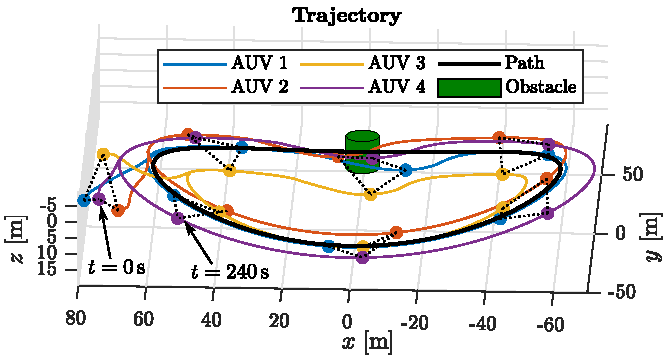
\includegraphics[width=0.75\textwidth]{figures/distr_NSB/sim_trajectory.pdf}
    \vspace{-4mm}
    \caption{The 3D trajectory of the AUVs. The markers represent the AUVs at times $t = 0, 40, \ldots, 240$ seconds. The dotted lines represent the communications graph.}
    \label{fig:distr_NSB_sim_trajectory}
\end{figure}
